\documentclass{article}
\usepackage{amsmath}
\usepackage{float}
\usepackage{amssymb}
\usepackage{graphicx}
\usepackage[margin=1in]{geometry}
\usepackage{multicol,caption,listings}
\usepackage{cite}
\usepackage[stable]{footmisc}

\bibliographystyle{plain}

\begin{document}

\title{Polymer Chain Monte Carlo}
\author{A. Lovell}
\maketitle

\noindent \textbf{Abstract}  Polymer chains are of great interest in biophysics, and while one might think to use a molecular dynamics calculation to simulate their configurations, for practical reasons, Monte Carlo techniques are more widely used.  In this project, we will use the Rosenbluth algorithm within a Monte Carlo framework to simulate polymer chains of varying lengths around $10^4$ atoms at several temperatures to investigate the correlation between the size of the polymer structure and the number of atoms within the chain.  This will be compared to theoretical models to investigate the systems we can create using a fixed distance between sequential atoms and the Lennard-Jones potential between all other pairs.

\begin{multicols}{2}

\section{Introduction}

Polymers are chains of atoms or molecules of the same type that interact directly between sequential atoms through a spring force and through all pairs via some other long- or short-range potential (given, for example, by hydrogen bonds, van der Waals interactions, or the Lennard-Jones interaction).  The typical number of atoms or molecules in a polymer is between $10^3$ and $10^5$ which can all be of the same type or different types.  \\

One would often think that a molecular dynamics calculation would be used to simulate a polymer chain.  In this case, the movement of the chain could be followed by calculating the forces between each pair of atoms for each time step and then used to update the chain's next position.  However, because of the different types of motion involved in the problem - ranging from fast motion of the individual atomic units to slow motion of the chain as a whole - this process can be inefficient, or even impossible, for long chains.  \cite{PhilNotes} Instead, Monte Carlo simulations are used to discover properties of the polymer.  \\

This report is broken up into the following sections.  In Section \ref{theory}, we will discuss the theory behind the problem, including the interaction between atoms and the algorithm that was used to run the Monte Carlo simulation.  Section \ref{IC} gives a brief discussion of the initial conditions of the simulation and a note on the units used in the calculation.  The results of the simulation are discussed in Section \ref{discuss}.  Finally, in Section \ref{concl}, we provide a summary of our work, along with further progress that could be made on this project in the future.  The appendix then provides some detail about our error calculations.  \\

\section{Theory}
\label{theory}

In the following section, we will describe some of the concepts that will be needed to simulate a polymer chain as well as briefly explain the path of the simulation code.

\subsection{Interaction}

The interactions between the atoms of polymer chains can be modeled in several ways.  One of the most common ways is to describe the interaction between sequential pairs of atoms as a stiff spring and put in a Lennard-Jones potential between every other pair of atoms.  \cite{PhilNotes}  However, in this project we will take a somewhat simplified approach.  Instead of stiff springs, we will fix the length between each successive pair of atoms (infinitely stiff springs), while keeping the interaction between all other pairs a Lennard-Jones interaction.  There are, of course, more complicated potentials that could be implemented to fold the polymer into more complex shapes (such as proteins or even origami ducks), but these will not be explored here.\\

The Lennard-Jones potential is 

\begin{equation}
\label{VLJ}
V_{LJ}(r) = 4\epsilon \left [ \left ( \frac{\sigma}{r} \right ) ^{12} - \left ( \frac{\sigma}{r}) \right ) ^6 \right ]
\end{equation}

\noindent where $\epsilon$ is the depth of the interaction, $\sigma$ is related to the particle size, and $r$ is the distance between the interacting pairs.  When the two atoms are far enough apart, they can be viewed as non-interacting.  For this reason, we would be able to introduce a cut-off radius beyond which the potential between two particles is taken to be zero.  \\

The form of (\ref{VLJ}) takes into account the short-range repulsive force between the two atoms due to Coulomb repulsion and the longer-range attractive forces from dipole-dipole and dipole-induced dipole forces.  \cite{verlet}  An example of the Lennard-Jones potential can be found in Figure \ref{VLJfig}.

\begin{figure}[H]
\begin{center}
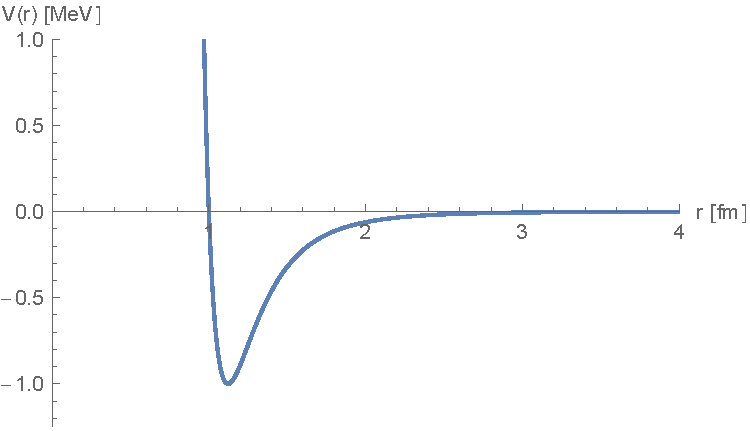
\includegraphics[width=\linewidth]{Figures/VLJ.pdf}
\caption{The shape of the Lennard-Jones potential.  Here, $\sigma=1$ fm (the distance where the potential crosses the r-axis) and $\epsilon =1$ MeV (the maximum depth of the interaction).}
\label{VLJfig}
\end{center}
\end{figure}

\subsection{Algorithm}
\label{RA}

In this Monte Carlo simulation, we build up the polymer chain by adding one atom at a time.  The algorithm that we use to pick the next atom's position is the Rosenbluth algorithm, proposed in 1956 by Marshall and Arianna Rosenbluth.  As compared to simple sampling - which generates all configurations with equal probability - the Rosenbluth algorithm generates configurations with different probabilities.  These probabilities cause the chain to be self-avoiding and to terminate when it is trapped in a configuration where every next possible addition would be on top of an already-placed atom.  \cite{Rosenbluth}  (This is a more straightforward concept for polymers created on a grid, which have a fixed number of nearest neighbors.)  \\

On a square (or cubic) lattice, this means that each nearest neighbor is tested as to whether or not it is already occupied, and the the probability that the next atom is placed at that site is based on the energy of the potential new configuration using the statistical factor

\begin{equation}
\label{prob}
P_i = \frac{1}{Z} e^{-V_i/T}
\end{equation}

\noindent where

\begin{equation}
\label{part}
Z = \sum \limits _{i=1}^{N_a} e^{-V_i/T}
\end{equation}

\noindent Here, $V_i$ is the potential energy between the $i^{th}$ candidate configuration and the rest of the chain, $N_a$ is the number of unoccupied nearest neighbors, and T is the temperature of the system.  These probabilities are mapped onto the range $[0,1]$, and a random number is picked within that same range.  If this random number falls within the range $P_i$, then the next atom is added at the position from which $V_i$ was calculated.  \\

However, we can also grow our polymer freely, without a grid.  In this case we have to sample from a circle in two-dimensions or a sphere in three-dimensions with the radius of the distance between each successive pair of atoms.  To do this, we sample from $\mathrm{cos}\theta \in [-1,1]$ and $\phi \in [0,2\pi]$ (taking $\theta = \pi/2$ for the two-dimensional case, to fix the third dimension).  This samples over the circumference of a unit circle in two-dimensions and the surface of a sphere in three-dimensions.  Some number, $N_a$, of points are randomly chosen, and new positions are calculated from

\begin{equation}
\begin{split}
x^{j}_i & = x^{j-1} + \mathrm{sin}\theta _i \mathrm{cos}\phi _i \\
y^{j}_i & = y^{j-1} + \mathrm{sin} \theta _i \mathrm{sin} \phi _i \\
z^{j}_i & = z^{j-1} + \mathrm{cos} \theta _i
\end{split}
\end{equation}

\noindent where we are placing the $j$th atom in the $i$th candidate configuration.  The probabilities for each $\textbf{r}_i$ to be chosen is the same as described above with equations (\ref{prob}) and (\ref{part}).

\subsection{Configuration}

The main quantity that we want to explore is the relationship between the size of the system and the number of atoms in the polymer, which should be related to the dimensionality of the simulation (e.g. two-, three-, or more dimensional space).  To do this, we relate the gyration radius, $R_g$, to the number of atoms in the chain, $N$, where 

\begin{equation}
\label{rg}
R_g^2 = \frac{1}{N} \sum \limits _{i=1}^{N} \langle (r_i - R_{cm})^2 \rangle
\end{equation} 

\noindent and 

\begin{equation}
\label{RNcomparison}
R \sim N^{\nu}
\end{equation}

The temperature, $T_{\Theta}$, defines the transition between a chain-like polymer ($T<T_{\Theta}$) and a dense, ball-like polymer ($T>T_{\Theta}$).  For temperatures below $T_{\Theta}$, $\nu = 1/ 2$, at $T_{\Theta}$, $\nu = 1/3$, and above $T_{\Theta}$, $\nu$ scales with the dimensionality of the simulation - namely, $\nu = 3/(d+2)$, where $d$ is the dimensionality of the simulation.  \cite{PhilNotes}\\

$R_g$ is the main observable we will be calculating for this Monte Carlo simulation.  From this, we can also define - or at least put some constraint on - the $\Theta $-temperature, $T_{\Theta}$.

\subsection{Code}

In this subsection, we will briefly describe the structure of the code and where the above ideas are implemented. \\

Initially, two atoms are placed at a distance of one unit length apart from each other.  The potential energy of the system is calculated.  To prepare to place the next atom, some number of points on the unit sphere are randomly chosen from a distribution of $cos\theta d\theta d\phi$.  The potential energy of each of these configurations is calculated, and the Rosenbluth algorithm, described in \ref{RA}, is implemented to choose the position of the next atom.  Once the next position has been chosen, the potential energy of the new system is calculated and the method repeats:  choose points on the unit sphere, implement the Rosenbluth algorithm, calculate the potential energy of the system.  \\

Once the entire chain (a given number of atoms, $N$) is constructed, the radius of gyration, from (\ref{rg}), is calculated for this polymer.  This chain-building process is repeated again and again to build up enough statistics to calculate a mean and and standard deviation (for the error).  

\section{Initial Conditions}
\label{IC}

The first two atoms of the chain were positioned at (0,0,0) and (1,0,0).  Essentially, these positions are arbitrary (only constrained to be 1 unit length apart), but it gives a good starting point for both the polymer on a grid and in free space.   Because this calculation is not performed on a grid, for each new position, 90 points on the unit sphere are tested.  This more easily prevents the chain from becoming stuck by only having options to place the next atom too close to previously placed atoms.  \\

In this calculation, we also chose $\epsilon =1$ and $\sigma=1$ for the Lennard-Jones potential parameters in (\ref{VLJ}).  In order to compare to data from the lab, we would just need to change our potentials to include realistic numbers for these two values.  Along with this, we also are using units where $k_B=1$.  This gives us temperature in eV, with $1$ eV $\approx 11600$ K.  Thus, even seemingly small temperatures quickly become large - and potentially unphysical.\\

\section{Discussion}
\label{discuss}

In this section, we present the main result of our calculation.  We were able to vary the temperature of the polymer, from 1.0 eV to 5.0 eV, as well as the number of atoms, $N=5000, 10000, 15000$, to calculate the radius of gyration and see how well our simulation compares to (\ref{RNcomparison}) for known values of $\nu$.  These results are summarized in Table 1 and the method of error, $\sigma_{R_g}$, calculation is discussed in the appendix.  \\

\begin{table*}
\begin{center}
\begin{tabular}{| c | c | c | c | c | c | c |}
\hline & $T=1.0$ eV &  & $T=2.0$ eV &  & $T=5.0$ eV & \\ \hline
 & \textbf{$log(R_g)$} & \textbf{$\sigma _{R_g}$} & \textbf{$log(R_g)$} & \textbf{$\sigma _{R_g}$} & \textbf{$log(R_g)$} & \textbf{$\sigma _{R_g}$} \\ \hline
$N=5000$ & 2.5119 & 0.343484 & 3.109664 & 0.312228 & 3.308621 & 0.330394 \\ \hline
$N=10000$ & 2.783211 & 0.295998 & 3.656107 & 0.335429 & 3.642807 & 0.321192 \\ \hline
$N=15000$ & 2.994968 & 0.376915 & 3.722428 & 0.343053 & 3.872835 & 0.318437 \\ \hline
\end{tabular}
\label{results}
\caption{Results for a three-dimension polymer chain in free space (not on a grid) for three different temperatures at three different polymer lengths.  Both the mean value ($log(R_g)$) and the standard deviation ($\sigma_{R_g}$) for each set of points is given.  Here, and throughout the report "log" means log base e - the natural log.}
\end{center}
\end{table*}

\begin{figure}[H]
\begin{center}
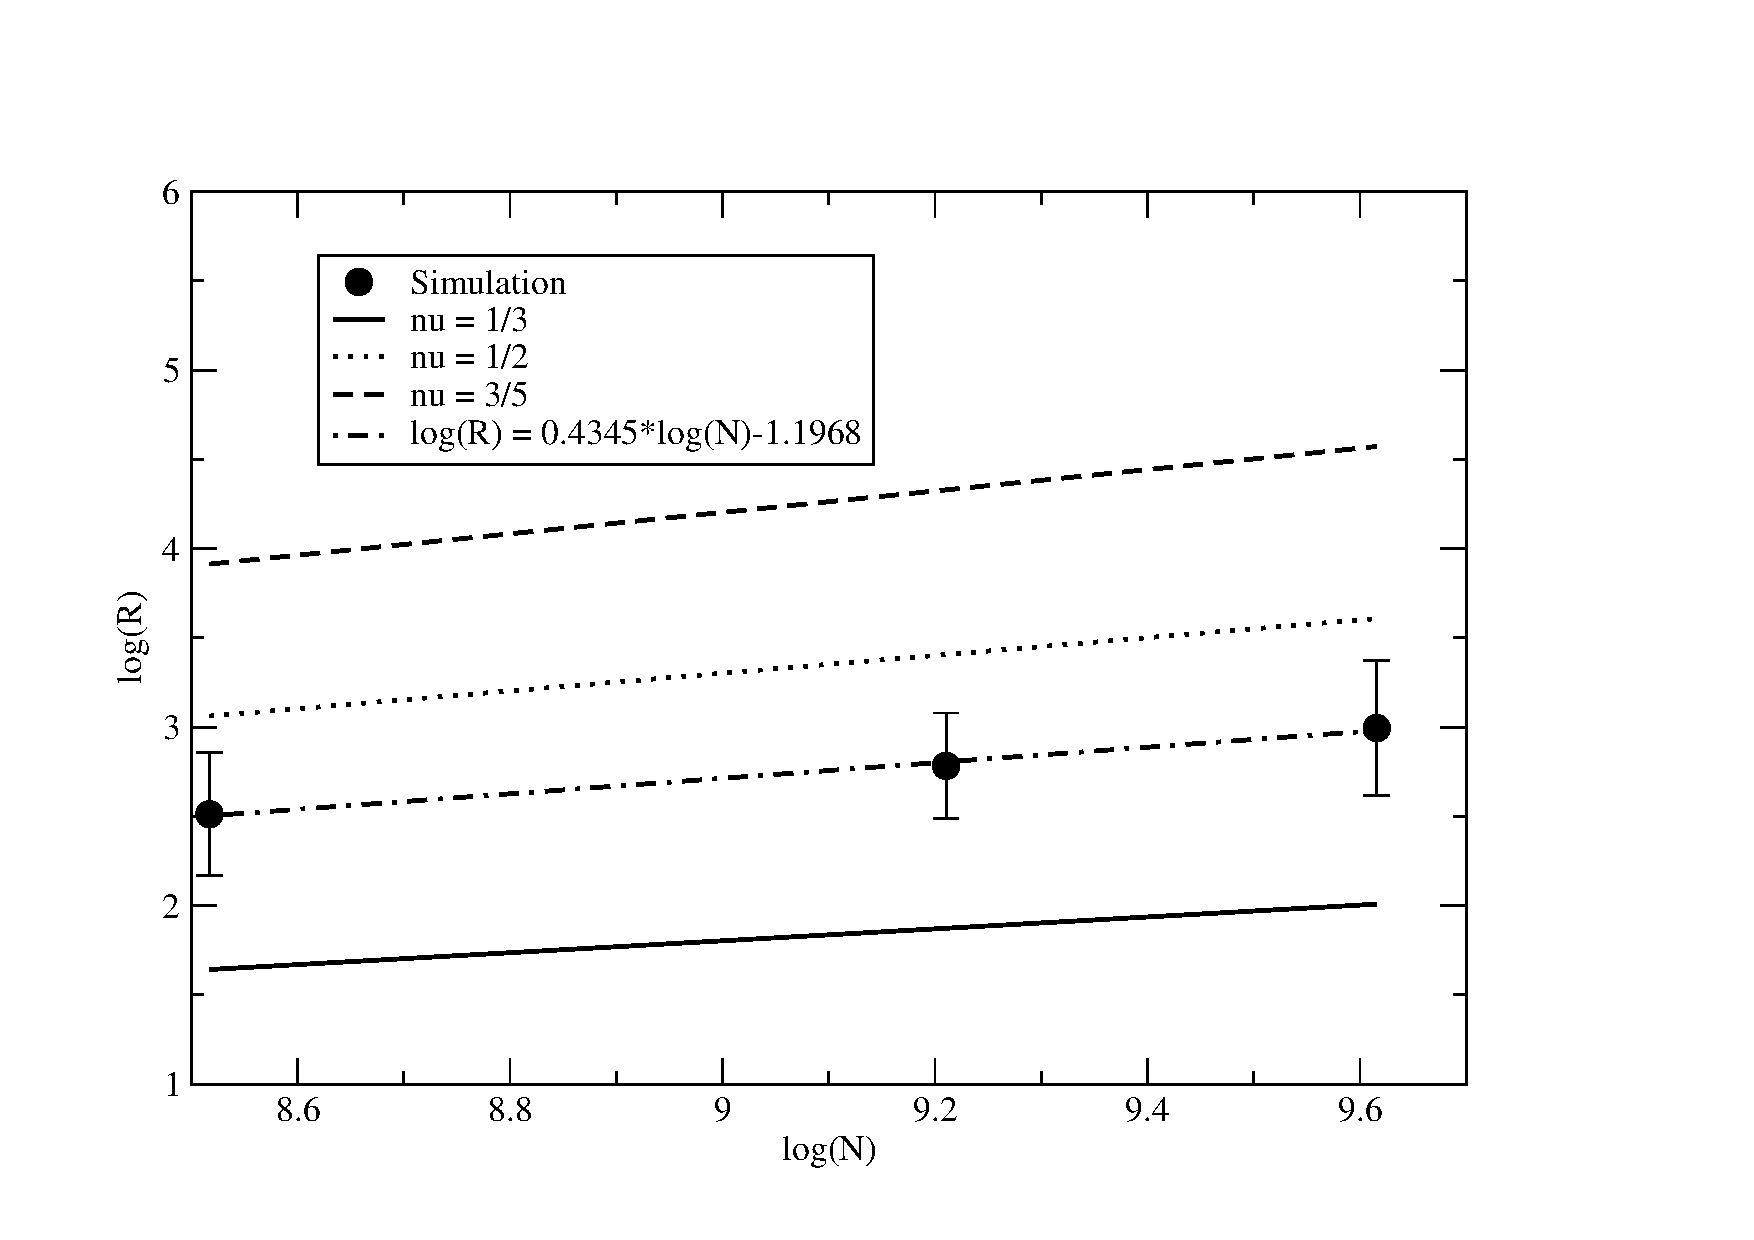
\includegraphics[width=\linewidth]{Figures/T1plot.pdf}
\caption{Results for $T=1.0$ eV.  Black dots give the Monte Carlo values calculated for this project, and the dotted-dashed line gives the best fit line through the simulation points.  The solid, dotted, and dashed lines show possible, interesting values of $\nu$ from (\ref{RNcomparison}).  Each of these three lines has the same y-intercept as the best fit line; thus, if one of these lines was the correct description of the simulation, it would go through the black dots and be aligned with the best fit line.}
\label{T1fig}
\end{center}
\end{figure}

In Figures \ref{T1fig}, \ref{T2fig}, and \ref{T5fig}, we show the results of the simulation plotted along with the best fit line for each set of data.  These fits are given in Table 2.  \\

\begin{figure}[H]
\begin{center}
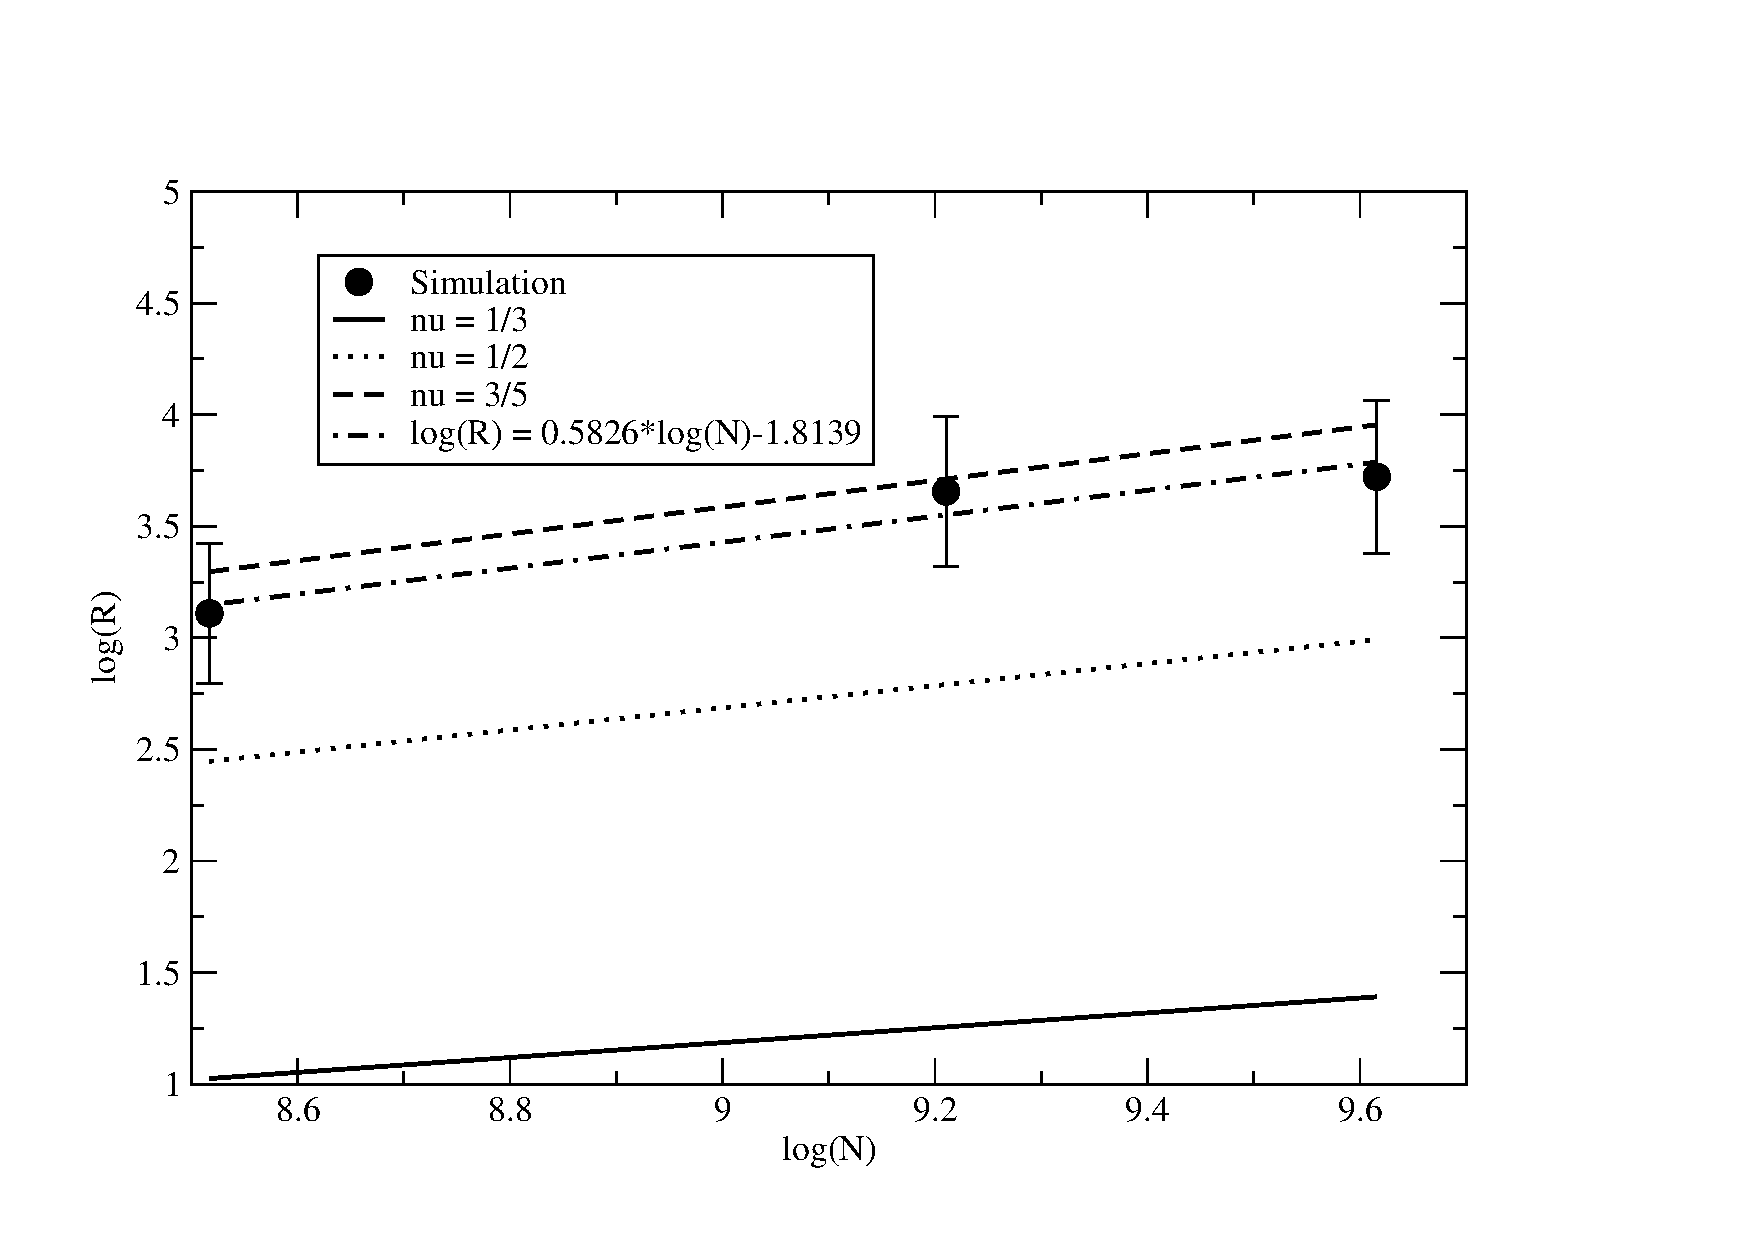
\includegraphics[width=\linewidth]{Figures/T2plot.pdf}
\caption{Same as Figure \ref{T1fig} but for $T=2.0$ eV.  We can see that $\nu = 3/5$ best describes the simulation.}
\label{T2fig}
\end{center}
\end{figure}

From these fits, we find that $\nu = 0.4345 \pm 0.03440$ for $T=1.0$ eV, $\nu = 0.5826 \pm 0.1642$ for $T = 2.0$ eV, and $\nu = 0.5102 \pm 0.02239$ for $T = 5.0$ eV.\footnote{These errors are discussed in more detail in the Appendix.}  The first two cases match up well with a temperature just below $T_{\Theta}$ for $T=1.0$ eV and for a temperature above $T_{\Theta}$ that follows the pattern $\nu = 3/(d+2)$ for $T = 2.0$ eV.  (Recall, for this simulation $d=3$ so $\nu = 0.6$.)  However, we see that for $T = 5.0$ eV, $\nu \approx 0.5$ which would seem to indicate that this is the $\Theta$-temperature. This cannot be the case.  To postulate an explanation for this, we note that $5.0$ eV $\approx 58000$ K, which is an order of magnitude hotter than the coolest part of the sun.  \cite{sun}  We assume that at these temperatures, our simple model is no longer valid, and we get nonsensical results from our calculations.  \\

From Table 2, we can also see that the $\chi^2$ value for each of these fits is extremely low.  This is a product of the fact that only three data points are being fit with by linear regression, causing a misleadingly small $\chi^2$ value.  Ideally, we want a $\chi^2$ value of 1 for every degree of freedom in the problem (e.g. $\chi ^2/dof =1$) which would indicate a perfect fit.  A very low $\chi ^2$, such as we have here, indicates that we have under-constrained our model by allowing too many free parameters for the number of data points. Thus, having run the simulation for more $N$ and $T$ values would serve to better constrain our fit, as well as give us more confidence that the parameters we calculated adequately described the results of our simulation.\\

\begin{figure}[H]
\begin{center}
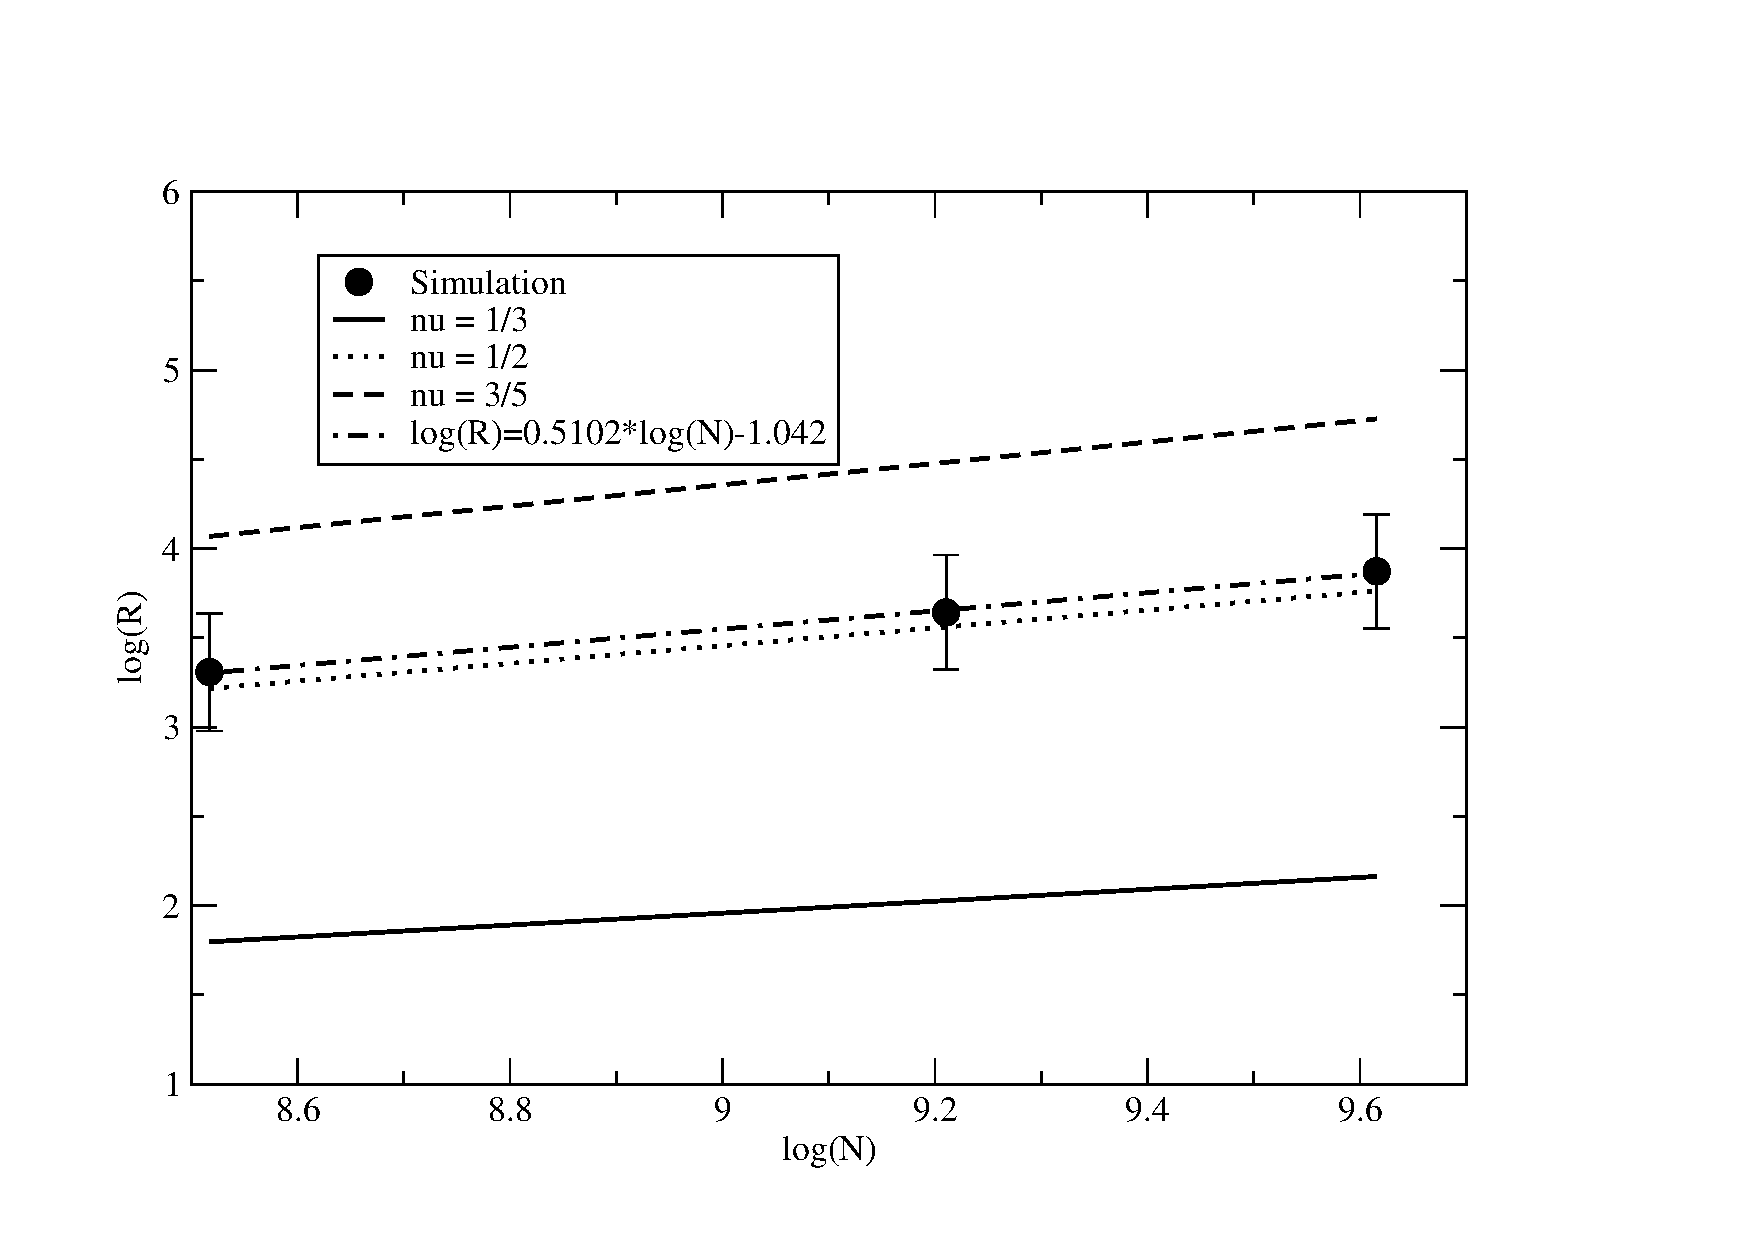
\includegraphics[width=\linewidth]{Figures/T5plot.pdf}
\caption{Same as Figure \ref{T1fig} but for $T=5.0$ eV.  We can see that $\nu = 1/2$ best describes the simulation.  This unexpected result is discussed more within the text.}
\label{T5fig}
\end{center}
\end{figure}

\begin{table*}
\begin{center}
\begin{tabular}{| c | c | c | c | c |}
\hline \textbf{T (eV)} & \textbf{m} & \textbf{b} & \textbf{s$_m$} & \textbf{$\chi ^2$} \\ \hline
1.0 & 0.4345 & -1.1968 & 0.03440 & 0.007327 \\ \hline
2.0 & 0.5826 & -1.8139 & 0.1642 & 0.1483 \\ \hline
5.0 & 0.5102 & -1.042 & 0.02239 & 0.003000 \\ \hline
\end{tabular}
\caption{Slopes ($m$) and y-intercepts ($b$) for the best fit lines for the simulation data in Table 1.  Best fit lines are given as $log(R_g) = m*log(N) + b$.  Here $log$ indicates the natural log.  In this case, the slope $m$ gives the value for $\nu$ from (\ref{RNcomparison}).  $s_m$ gives the error on the fit - only describing the difference between the values calculated from the fit and the simulation values, and $\chi^2$ takes into account, somewhat, the error from the simulation.}
\end{center}
\end{table*}

We can see from Figures \ref{T1fig}, \ref{T2fig}, and \ref{T5fig} that the error bars are significant for the range of data displayed.  These large errors did not decrease with the number of statistics, a trend which can be seen in Table 3.  From these figures, we can see that these large errors contribute to some uncertainty around the slope of the best fit lines, as the calculated value for $\nu$ does not take into account the error from the original simulation.  This uncertainty makes it unclear as to whether or not we can confidently describe the behavior of the chain.  Even though the best fit lines have a very low $\chi ^2$ value, this value is misleading, as described previously.    \\
  
\begin{table*}
\begin{center}
\begin{tabular}{| c | c | c | c |}
\hline & $T=1.0$ eV & $T = 2.0$ eV & $T = 5.0$ eV \\ \hline
$N=5000$ & 64 (0.343484) & 500 (0.312228) & 1000 (0.330394) \\ \hline
$N=10000$ & 43 (0.295998)  & 500 (0.335429) & 810 (0.321192) \\ \hline
$N=15000$ & 45 (0.376915) & 290 (0.343053) & 1147 (0.318437) \\ \hline
\end{tabular}
\caption{Number of chains produced for each combination of number of atoms in the chain (first column) and temperature (top row).  The number in parentheses gives the error calculated for each of these points, also given in Table 1.  It is clear to see that the errors do not decrease as the number of calculations increases, even though, in some cases, the number of simulations increases by orders of magnitude.}
\end{center}
\end{table*}

Still, in the region where our simulation is valid, we have calculated reasonable results for our three-dimensional simulation of a polymer chain, even if the error analysis leaves somewhat of a question as to the behavior of the chain at our various temperatures of interest.   \\

\section{Conclusion}
\label{concl}

In this work, we were able to construct a Monte Carlo simulation of a three-dimensional polymer chain of approximately $10^4$ atoms at temperatures of 1.0 eV, 2.0 eV, and 5.0 eV.  The polymer was simulated without being confined to a grid.  By comparing the natural logarithm of the gyration radius and number of atoms in the chain, we were able to discover properties of the chain itself and find the exponent, $\nu$.  We found that $\nu = 0.4345 \pm 0.03440$ for $T = 1.0 $ eV, $\nu = 0.5826 \pm 0.1642$ for $T =2.0$ eV, and $\nu = 0.5102 \pm 0.02239$ for $T=5.0$ eV.  Through this, we were able to compare to known behavior above and below the $\Theta$-temperature.  \\

However, there is still future work that can be accomplished.  While we calculated a polymer chain in three-dimensions, it would also be interesting to calculate higher (or lower) dimensional chains and examine the scaling of the size of the chain with the number of atoms added to the chain, $\nu$.  The same scaling ($\nu = 1/3$ below $T_\Theta$, $\nu = 1/2$ at $T_\Theta$, and $\nu = 3/(d+2)$ above $T_\Theta$) should hold, but it would be an interesting project nonetheless to generalize the code.  It would also be interesting to examine the differences between this type of self-avoiding walk that is not confined to a grid and a self-avoid walk confined to a cubic grid (or other shape grid).  From this, we could see how the dimensionality affects various grids on which the chain is created.  For all of this, we could also run the calculation in smaller temperature steps to find the $\Theta$-temperature.  \\

There are also several thermodynamical quantities that could be calculated from this system, including specific heat and thermal energy.  We could also change the interaction between the atoms within each chain.  Although we used a fixed bond length between each successive atom and a Lennard-Jones interaction between all pairs of atoms, there are other interactions that could describe a more realistic polymer, including using a stiff spring to model the interaction between successive atoms instead of a fixed bond length.  We also could have changed the strength (and type) of the interaction between various pairs to see what kinds of shapes we could form with our polymer chain.  \\

There have also been developments within the last two decades of the Pruned-enriched Rosenbluth method which combines the Rosenbluth method with recursive enrichment.  This algorithm allows for simulations of up to $N=10^6$ atoms in a single chain with high statistics, applicable to calculations both on and off of a lattice.  \cite{PERM}  In future work, this could be an interesting algorithm to implement, especially if it is more efficient and can give higher statistics in a shorter amount of time than the original Rosenbluth algorithm.  \\

Still, without all of this, we were able to model a polymer chain of $10^4$ atoms in three-dimensions without a grid.  \\

\appendix

\section{Error Analysis}

Just as experimentally measured data points should quote errors - whether due to systematics, timing, or unknown quantities - theoretical simulations and calculations should also give error bars.  To do this, we run our simulation several times to find a mean value and a standard deviation.  The mean is calculated by

\begin{equation}
\bar x = \frac{1}{N} \sum \limits _{i=1}^N x_i
\end{equation}

\noindent where $\bar x$ is the mean value, $x_i$ are the values of a given quantity from each calculation (for instance the length of the chain), and $N$ is the number of simulations that were performed.\\

To find the error on each data point, we average the standard deviation for each run.

\begin{equation}
\label{stddev}
\sigma _x^2 = \frac{1}{N} \sum \limits _{i=1} ^N (x_i - \bar x)^2
\end{equation}

\noindent Here, $\sigma _x$ is the error for the variable $x$ from each calculation.  We can see that the errors decrease as $1/\sqrt{N}$.  \\

Because we are calculating a fit to data, we should also report a $\chi ^2$ value for that fit, to assess its "goodness" - or the quality of the fit when compared to data.  \cite{Nunes}  In this case, we would calculate the $\chi^2$ of each of the linear fits that are made to the simulation data.

\begin{equation}
\chi ^2 = \sum \limits _{i=1} ^N \frac{(x^{sim} - x^{fit})^2}{\sigma _x ^2}
\end{equation}

\noindent In this case, $x^{sim}$ is the parameter value from the simulation, $x^{fit}$ is the parameter value from the fit through the simulation data, and $\sigma _x ^2$ is the square of the standard deviation (the variance) from (\ref{stddev}). \\

Although this does not give us an error on the fits that are being made, it does give some indication as to the quality of the fit.\\

Using similar ideas, errors for the fits can be calculated (although these errors still do not take into account the error from the simulations).  For these errors (such as those in Table 1), we take

\begin{equation}
s^2 = \frac{1}{n} \sum \limits _{i=1} ^{n} (y^{data}_i - y^{fit}_i)^2
\end{equation}

\noindent where $s$ is the error on the fit, $n$ is the number of data points fit, $y^{data}$ is the result of the simulation, and $y^{fit}$ is the result from the fit (both calculated at the same point).  \cite{staterr}

\end{multicols}

\bibliography{chainbib}

\end{document}